\section{Diskussion}
\label{sec:Diskussion}

\subsection{Anregung durch eine Rechteckspannung}

Der theoretisch zu erwartende Wert für die Zeitkonstante ist $\tau _\text{theo}=\SI{1.405(56)}{\milli\second}$, der aus dem 
ersten Teil des Experiments ermittelte ${\tau _\text{exp}=\SI{0.82(1)}{\milli\second}}$. 
Da der experimentelle Wert deutlich außerhalb des Fehlerintervalls von $\tau _\text{theo}$ liegt, kann an dieser Stelle 
nicht von einer statistischen Abweichung ausgegangen werden. 
Der Fehler kann auch nicht an nicht berücksichtigten Innenwiderständen der Geräte oder an ohmschen Verlusten der Kabel 
liegen. 
Wahrscheinlicher ist ein systematischer Messfehler, der sich im Nachhinein nur schwerlich zu finden lässt. 
Möglichkeiten könnten überdrehte -- und deshalb keine richtig skalierenden -- Knöpfe am Oszilloskop sein, sodass alle 
abgelesenen Spannungswerte um einen Faktor verschieden von der tatsächlich angelegten Spannung sind. 

\subsubsection{Frequenzabhängigkeit}
Vor allem bei Frequenzen im höheren Bereich ist es hilfreich, den externen Trigger des Oszilloskops zu nutzen, um zeitaufwändige Kalibrierungen zu vermeiden.
In Abbildung \ref{fig:mess_b_c} sind die drei Größenordnungen der Frequenzsprünge sehr gut erkennbar. Auch lässt sich der exponentielle Verlauf beider Messkurven
sehr gut ablesen. Die Größe der Amplitude konvergiert mit steigender Frequenz gegen null, was zu erwarten ist und aus Gleichung \eqref{eqn:ampl_omega} bereits hervorgeht.
Die Phasenverschiebung konvergiert erwartungsgemäß gegen $\sfrac{\pi}{2}$, was an der Natur des Arkustangens liegt.
Mit den gegebenen Werten $R = \SI{15.058}{\kilo\ohm}$ und $C = \SI{93.3}{\nano\farad}$ errechnet sich nach Gleichung \eqref{eqn:phas_diff_omega} für $f = \SI{2112}{\hertz}$ eine Phasenverschiebung
von $arctan(15058\cdot93.3\cdot10^{-9}\cdot2112\cdot2\pi) \approx 1.517$. Im Vergleich: $\sfrac{\pi}{2} \approx 1.57$. Der tatsächliche Messwert bei dieser Frequenz liegt bei 
$\symup{\Delta\varphi} \approx 1.357$. Eine mögliche Erklärung für die kleine Differenz zwischen dem erwarteten und dem gemessenen Wert sind innere Widerstände
der Messtechnik und des Generators. Zudem können die Angaben der Bauteile von den wahren Werten abweichen.

\subsection{Integrieren der Generatorspannung}

Bei allen drei Spannungen kann sehr gut die Phasenverschiebung um $\sfrac{\pi}{2}$ beobachtet werden, die wenn überhaupt 
nur minimal kleiner ist. 
Dies ist konsistent mit der Theorie, da nur für eine unendlich große Frequenz eine solche Phasendifferenz bewerkstelligt 
werden kann. Eine im mathematischen Sinne unendlich große Frequenz ist selbstredend in der Praxis nur näherungsweise zu 
realisieren. 

Bereits bei der Durchführung fällt auf, dass die Skala der Kondensatorspannung stark vergrößert werden muss, um Amplituden 
vergleichbarer Größenordnung auf dem Oszilloskop beobachten zu können. 
Dies rührt daher, dass bei hoher Frequenz ein vergleichsweise sehr kleiner Anteil der Spannung beim Kondensator ankommt, 
wie in der Theorie ausführlich erklärt wird. 

\begin{figure}
\centering
\begin{subfigure}{0.48\textwidth}
    \centering
    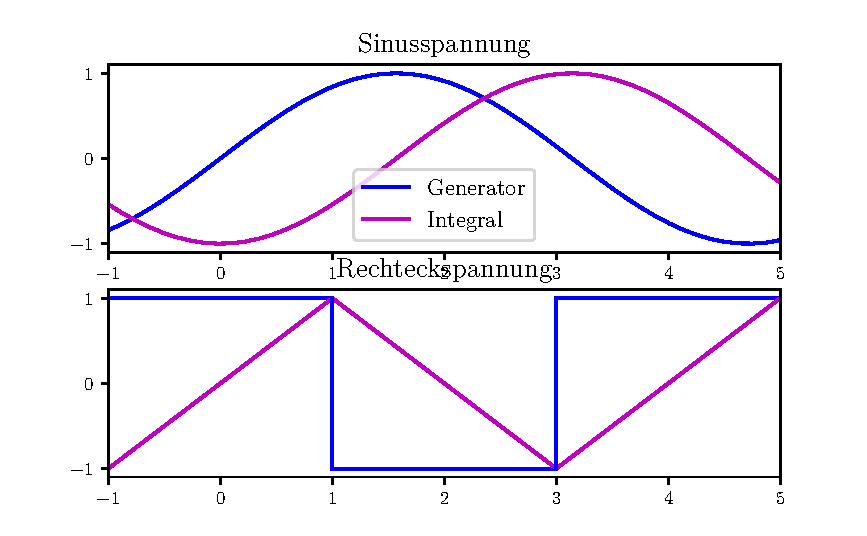
\includegraphics[height=5cm]{plots/erwart_int1.pdf}
    \label{fig:erw1}
\end{subfigure}
\begin{subfigure}{0.48\textwidth}
    \centering
    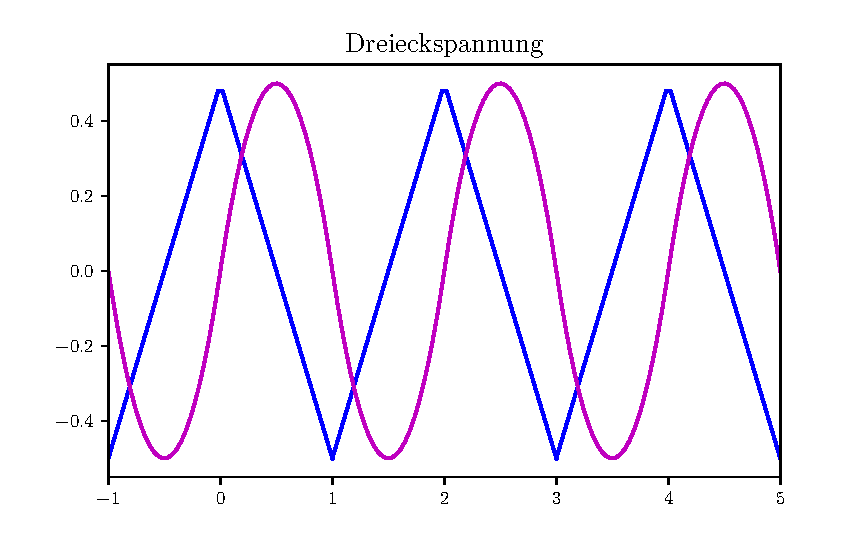
\includegraphics[height=5cm]{plots/erwart_int2.pdf}
    \label{fig:erw2}
\end{subfigure}
\caption{Die Spannungskurven und ihre zugehörigen Integrale.}
\label{fig:int}
\end{figure}

Um die Bilder vom Oszilloskop gut vergleichen zu können, sind in \ref{fig:int}  
die jeweiligen Spannungsarten mit zugehörigen Funktionsgraphen abgebildet, deren Ableitung die Spannungskurve ergibt. 
Der Übersicht halber wird an dieser Stelle auf eine explizite Darstellung der Funktionsdefinitionen von Dreiecks- und Rechteckskurven 
und deren Integrationen verzichtet. Sie bestehen aus trivialen linearen stückweise stetigen beziehungsweise differenzierbaren 
Funktionen. 

Wie durch einen Vergleich der Abbildungen klar ersichtlich ist, entsprechen die theoretischen Überlegungen bezüglich der 
integrierenden Eigenschaft eines RC-Kreises den experimentellen Beobachtungen. 